\documentclass[aspectratio=169]{beamer}


\usepackage{ccicons}
\usepackage{import}
\usepackage[yyyymmdd]{datetime}
\renewcommand{\dateseparator}{-}
\usepackage{marvosym}
\usepackage{xcolor,colortbl}
\usepackage[prefix=]{xcolor-material}
\usepackage{pifont}
\usepackage{hyperref}
\usepackage{mathtools}

\newcommand{\linegap}{\par\addvspace{3ex}}
\newcommand{\linegapgap}{\linegap\mbox{}\linegap}
% \newcommand{\linegap}{\mbox{}\\\mbox{}\\}
\newcommand{\pausegap}{\pause\linegap}
\newcommand{\pausegapgap}{\pause\linegapgap}
\newcommand{\pausenl}{\pause\par}

\newcommand{\emf}[1]{\textcolor{red}{#1}}
\newcommand{\gemf}[1]{\textcolor{green!50!black}{#1}}
\newcommand{\cmark}{\gemf{\ding{51}}}
\newcommand{\xmark}{\emf{\ding{55}}}

\setbeamersize{text margin left=5pt,text margin right=5pt}
\setbeamertemplate{theorems}[numbered]
\setbeamercolor{footlinecolor}{fg=blue,bg=white!85!black} 

\setbeamertemplate{navigation symbols}{%
    \usebeamerfont{footline}%
    \vspace*{-3pt}
    \begin{beamercolorbox}[wd=\paperwidth,dp=1ex]{footlinecolor}
      \hrule
      \vspace*{1pt}
      \mbox{}\;
      % \href{http://creativecommons.org/licenses/by-nc-sa/4.0/}{\ccbyncsa}
      % \dev{Development version}
      % \hfill
      TechConnect~\the\year\hfill
      \insertshortauthor
      \hfill
      \insertshortinstitute\hfill
      \insertpagenumber%\insertframenumber
      \;\;
    \end{beamercolorbox}%
    \hspace{0.5pt}
  }
  
\title{Towards Trustworthy AI}
\author{\gemf{Ashutosh Gupta} and S. Akshay}
\institute{CSE department, IIT Bombay}
% \institute{IIT Bombay\\
% SBI Foundation Hub project}
\begin{document}
\maketitle

\begin{frame}
  \begin{center}
    \Huge
  {Why do we need to check AI for \gemf{trust}?} 
  \end{center}
\end{frame}

% \begin{frame}
%   \begin{center}
%     \Huge
%   {What is AI?}      
%   \end{center}
% \end{frame}


\begin{frame}
  \frametitle{Problems and algorithms}
  \begin{minipage}{0.6\linewidth}
  Consider problems
  \begin{itemize}
  \item Sorting an array
  \item Route search in GMaps
  \item Finding arbitrage among stocks
  \end{itemize}    
  We usually have algorithms to solve the problems.
  \end{minipage}
  \begin{minipage}{0.38\linewidth}
  \begin{center}
    
\includegraphics[height=4cm]{images/directions}    
  \end{center}    
  \end{minipage}
  \pausegap
  \begin{center}
    {\Huge
      Input $\rightarrow$ Algorithm $\rightarrow$ Output
    }    
  \end{center}  
\end{frame}

\begin{frame}
  \frametitle{Problems without clear description}
  \begin{minipage}{0.6\linewidth}
  Consider problems:
  \begin{itemize}
  \item Loan dispersal
  \item Fraud detection
  \item Face recognition    
  \item ChatBots
  \end{itemize}
  \end{minipage}
  \begin{minipage}{0.38\linewidth}
    \begin{center}
    
\includegraphics[height=3cm]{images/face}    
  \end{center}    
  \end{minipage}
  \pausegap
  No \emf{\em known} algorithm to solve the problem but we have some \emf{\em rough} ideas about their behavior.
  \pausegap
  \begin{example}
    A loan dispersal program should follow the following rule among many other rules.
    \begin{center}
      If someone has a lot of assets, give them a loan.
    \end{center}    
  \end{example}
\end{frame}

\begin{frame}
  \frametitle{AI Model}
  AI models turn our rough understanding into a computer program.
  \begin{center}
    {\Huge
      Input $\rightarrow$ AI Model $\rightarrow$ Output
    }    
  \end{center}
  \pausegap
  We {\em train} AI models by showing them a list of input and output pairs.
  \pausegap
  The AI model is a computer program that \emf{approximates} the \gemf{ideal algorithm}.
  \pausegap
  The \gemf{ideal algorithm} is \emf{unknowable}.
\end{frame}

\begin{frame}
  \frametitle{Approximation: \gemf{Good}, Bad, and Ugly}
  Good: approximations are essential to build AI models.
  \linegap
  \begin{center}
    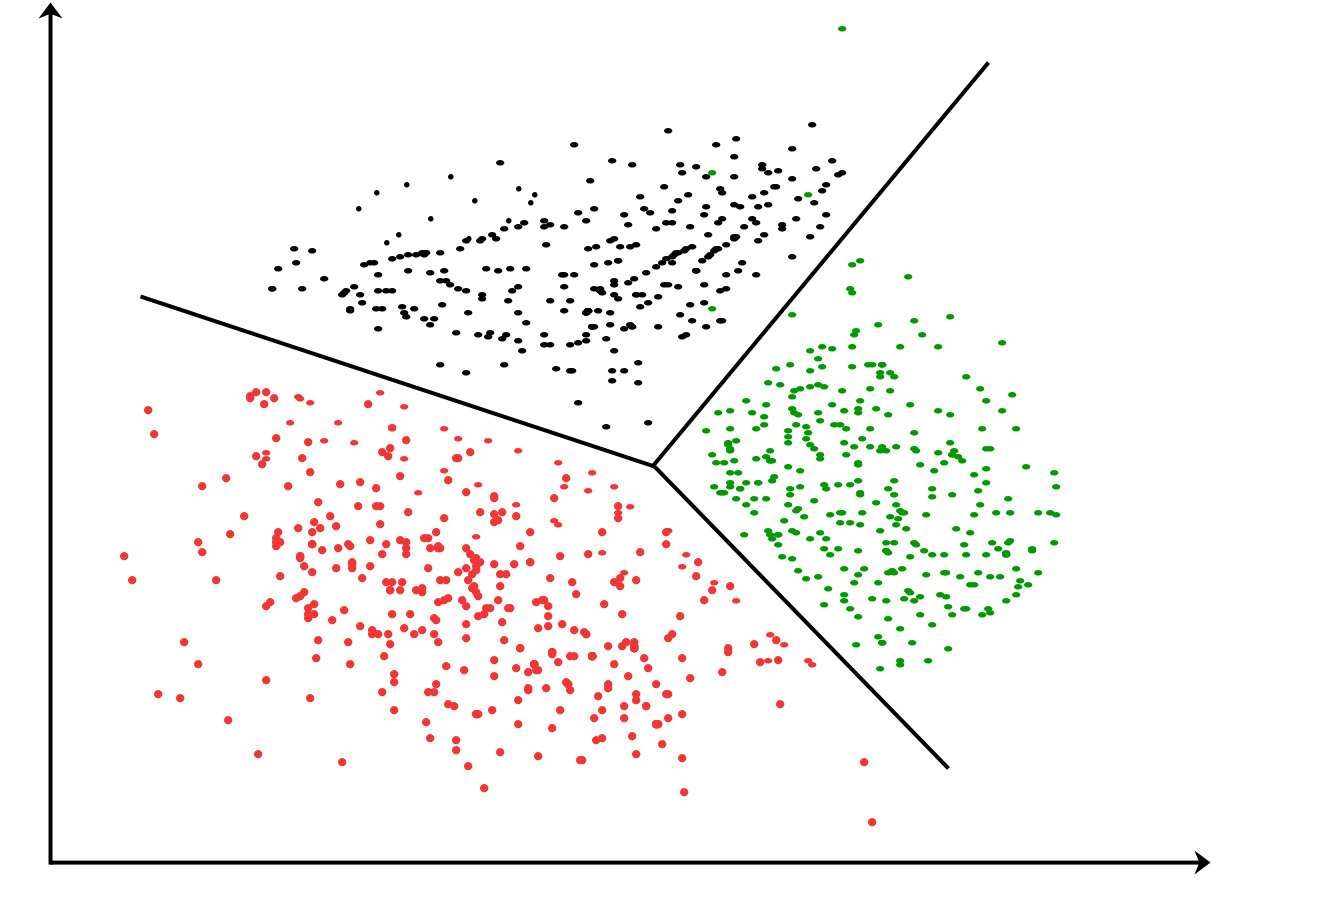
\includegraphics[height=3cm]{images/clustering}    
  \end{center}      
  \pausegap
  \begin{example}
    Deciding: who is loan worthy?
  \end{example}
  \pausegap
  Someone has to draw a line in the sand!
\end{frame}

\begin{frame}
  \frametitle{Approximation: Good, \gemf{Bad}, and Ugly}
  ``Bad'': AI Models are \gemf{expected} to have limited accuracy.
  \linegap
  \begin{center}
    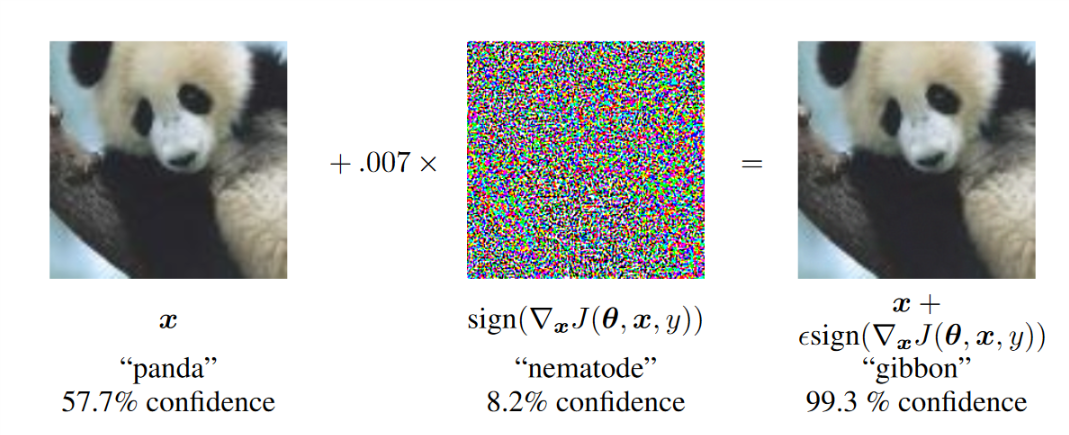
\includegraphics[height=3cm]{images/error}    
  \end{center}
  Actually, it is a good thing about AI!
\end{frame}

\begin{frame}
  \frametitle{Approximation: Good, Bad, and \emf{Ugly}}
  Ugly: AI Models may fail catastrophically when deployed in mission-critical applications.
  \linegap
  \begin{center}
    
\includegraphics[height=3cm]{images/tesla}    
  \end{center}
  \pausegap
  \begin{center}
  {\Huge
   Can we avoid UGLY? 
  }    
  \end{center}
\end{frame}

\begin{frame}
  \begin{center}
    \Huge
    {Avoiding ugly: you need formal methods }
  \end{center}
\end{frame}

\begin{frame}{Formal methods}
  % \begin{itemize}
% \item
  A technology dealing with providing strong guarantees to computing systems
  % \end{itemize}
  \pausegap
  We search for bugs in \gemf{all corners} of the system.
  \pausegap
  Since systems are \emf{complex and large}, the search \gemf{needs to be clever}.
\end{frame}

\begin{frame}{Where is it used?}
  \begin{block}{Industry use cases}
    Commonly used in Software and Hardware systems
  \end{block}
  \pausegap
  Since the technology is expensive, it is used \emf{only} in high-stakes systems.
  \begin{itemize}
  \item Cockpit of airplanes
  \item Cloud infrastructure of Amazon
  \item Correctness of SMART contracts
  \end{itemize}
\end{frame}

\begin{frame}{Can we extend this to AI systems?}
  AI components are being deployed everywhere in the economy.
  \pausegap
  Including, where the stakes are high, e.g., DigiYatra.
  \pausegap
  \begin{itemize}
  \item Rich area of current research
  \item Many research papers and active work
  \end{itemize}
  \end{frame}

\begin{frame}
  \begin{center}
    \Huge
    {An example: 
      problem of sensitivity}
     % \\
     %    \pause
     %    \Large Our Focus
  \end{center}
\end{frame}

\begin{frame}
  \frametitle{Example Problem Statement: sensitivity of a loan dispersal model}
  \begin{itemize}
  \item To give formal guarantees, we need to first define the problem mathematically.
  \item What is the input?
  \end{itemize}  
\end{frame}

\begin{frame}
  \frametitle{Example Problem Statement: sensitivity of a loan dispersal model(2)}
  \begin{block}{Input}
    \begin{itemize}
    \item A feature space $\mathcal{F}$, fields you fill in the application form, e.g.,
      \begin{itemize}
      \item Age, Address, Salary, etc.
      \end{itemize}
      \pausegap
    \item A decision model $X$ (trained by the user!) over $\mathcal{F}$
      \begin{itemize}
      \item $X$ takes a loan application as input $v$ and gives a decision.
      \item e.g., $X: Loan Application \rightarrow Yes/No$
      \end{itemize}
      \pausegap
    \item The set of \gemf{sensitivity} features that you are interested in $F\subseteq \mathcal{F}$, e.g.,
      \begin{itemize}
      \item Age, Gender, etc.
      \end{itemize}
    % \item Optional: dependency between features.
    \end{itemize}
  \end{block}
\end{frame}

\begin{frame}
  \frametitle{Example Problem Statement: sensitivity of a loan dispersal model(3)}
  \begin{block}{The sensitivity problem}
    Given the model $X$ and feature set $F\subseteq \mathcal{F}$, are there two loan applications $v_1,v_2$ such that
    \begin{itemize}
    \item $v_1$ and $v_2$ differ only on $F$ (same on all the other features)
    \item but, outputs/decisions are different, i.e., $X(v_1)\neq X(v_2)$.
    \end{itemize}
    % $|F|$ can be 1 or more... but typically small.
  \end{block}
  \pausegap
  \begin{example}
    Is it possible to change the decision of the model by only changing the age?
    % Is it possible in \emf{\Huge any} loan application to change the decision of the model by only changing the age?
    % Is it possible to change the decision of the model by only changing the age
    % in \emf{\Huge all} applications?
  \end{example}
\end{frame}

% \begin{frame}{A more nuanced problem statement}
%   As written above, the statement is too precise! We will always answer insensitive!
%   \pause
%   \begin{block}{The sensitivity problem}
%     Given the model $X$ and feature set $F\subseteq \mathcal{F}$, and thresholds $\epsilon$ and $\delta$,
%     are there two inputs $v_1,v_2$ such that
%     \begin{itemize}
%     \item $v_1$ and $v_2$ differ on $F$ by some small threshold $\epsilon$
%     \item but, outputs/decisions are different by more than $\delta$, i.e., $|X(v_1)-X(v_2)|>\delta$.
%     \item such that the dependencies between features are maintained. 
%     \end{itemize}
%   \end{block}
 
% \end{frame}

\begin{frame}
  \frametitle{What do we find?}
  We developed the algorithms and tools for finding sensitivity.
  Here is an example of a sensitive model from a benchmark.
  \begin{center}
    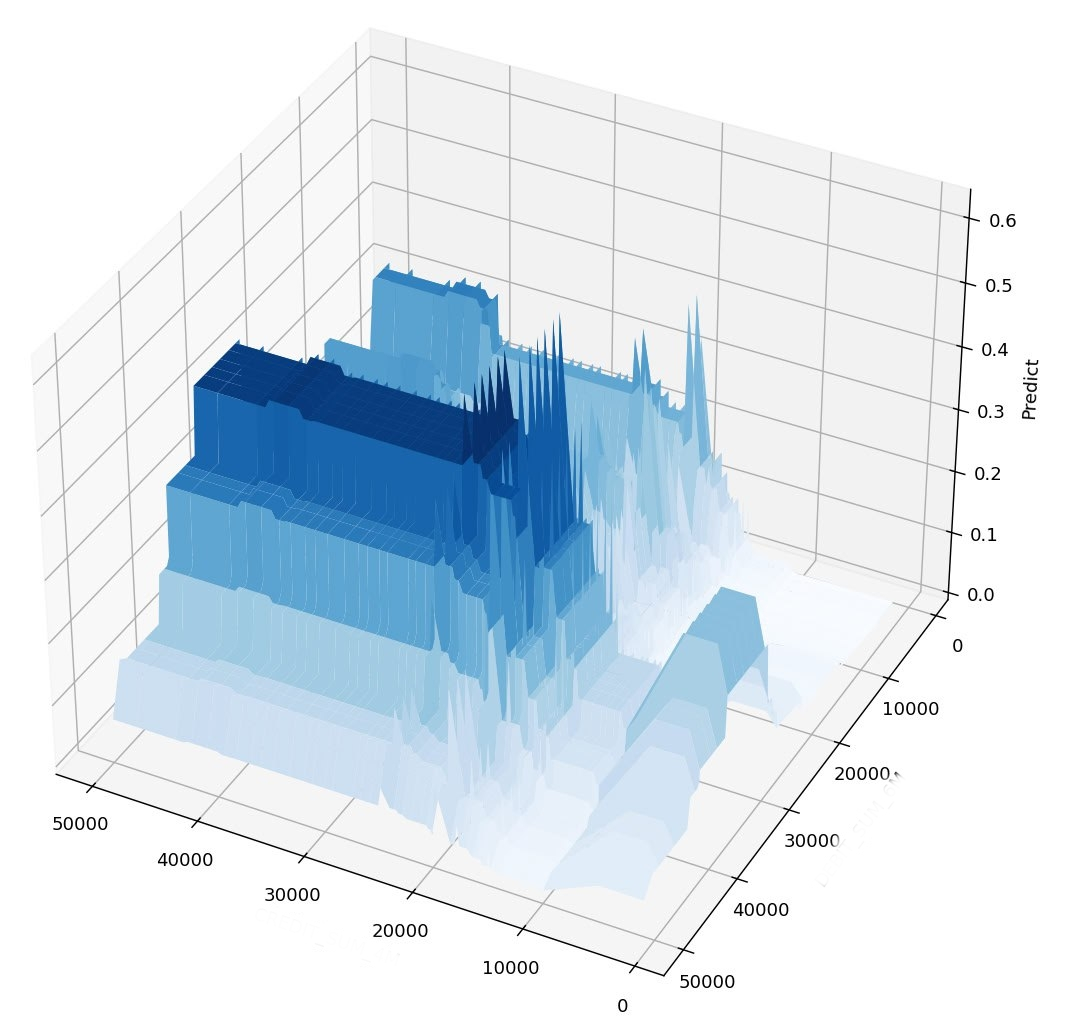
\includegraphics[height=6cm]{images/glitch-clean}    
  \end{center}
  \pause
  \vspace{-3mm}
  The model is not as large as LLMs. Today, LLMs are too large to perform a similar analysis. 
  % The above result is on of the models 
\end{frame}

\begin{frame}
  \frametitle{Conclusion}
  \begin{itemize}
  \item We need to develop methods to audit AI systems
    \linegap
  \item Technology exists that can analyze small to mid-size AI systems
    \linegap
  \item Call to action: develop analysis technology that scales to large AI systems/models
  \end{itemize}
\end{frame}

% \begin{frame}
%   \begin{center}
%     \Huge
%   {Solver technology}      
%   \end{center}
% \end{frame}


% \begin{frame}
%   \frametitle{Example: satisfaction}
%   Let $x,y$ be \gemf{rational variables}.
%   \pausegap
%   Choose a \gemf{value} of $x$ and $y$ such that the following \gemf{formula} holds true.
%   \linegap
%   \hspace{3.8ex}$x + y = 3$
%   \pausegap
%   We say
%   $$
%   \{x \mapsto 1 , y \mapsto 2 \} \models x + y = 3.
%   $$
%   % \mycallout{10mm}{(58mm,62mm)}{(0mm,4mm)}{4}{model}
%   % \mycallout{12mm}{(85mm,62mm)}{(0mm,4mm)}{5}{formula}
%   % \comment{
%   %   $x$ and $y$ are not rational numbers.
%   %   They are variables, i.e, symbols that can hold numbers.
%   %   A model is an assignment to the variables of the formula.
%   %   $m \models F$ is read as `$m$ satisfies $F$`.
%   % }
% \end{frame}


% % \begin{frame}
% %   \frametitle{Evaluation}
% %   For a given model $m$ and formula $F$,
% %   \begin{center}
% %     \Huge
% %     $m \models F$?
% %   \end{center}
% %   \pause
% %   \begin{ex}
% %     $$
% %     \{x \mapsto 1 , y \mapsto 2 \} \models x + y = 3.
% %     $$
% %     % \mycallout{10mm}{(43mm,45mm)}{(0mm,4mm)}{3}{model}
% %     % \mycallout{12mm}{(70mm,45mm)}{(0mm,4mm)}{4}{formula}
% %   \end{ex}
% %   \pause
% %   \begin{exercise}
% %     \begin{itemize}
% %     \item $\{x \maps 1 \} \models x > 0$?\qquad\answer{\cmark}
% %     \item $\{x \maps 1, y \maps 2 \} \models x + y = 3  \land x > 0$?\qquad\answer{\cmark}
% %     \item $\{x \maps 1, y \maps 2 \} \models x + y = 3   \land x > 0 \land y > 10$?\qquad\answer{\xmark}
% %     \end{itemize}    
% %   \end{exercise}
% %   \begin{exercise}
% %     Can we say something more about the last formula?
% %   \end{exercise}
% % \end{frame}

% \begin{frame}
%   \frametitle{Satisfiablity problem {\em aka.} SAT problem}
%   Satisfiability == Is there any model?
%   \vspace{-3mm}
%   \begin{center}
%     \Huge
%     Is $F$ SAT?
%   \end{center}
%   % \pausenl
%   % Harder problem!
%   \pause
%   \begin{example}
%     Are the following formulas sat?
%     \begin{itemize}
%     \item $x + y = 3  \land x > 0$\pause\qquad{\cmark}
%     \item $x + y = 3   \land x > 0 \land y > 10$\pause\qquad{\xmark}
%     \item $x > 0 \lor x < 1$\pause\qquad{\cmark}
%     \end{itemize}
%   \end{example}
% \end{frame}


% \begin{frame}
%   \frametitle{Example: SAT problem(contd.)}
%   \vspace{-3ex}
%   Let $x,y$ be rational variables.
%   \par
%   Choose a \gemf{value} of $x$ and $y$ such that the following \gemf{formula} holds true.
%   \linegap
%   \hspace{3.8ex}$x + y = 3 \pause \land y > 10 \pause \land x > 0$ \hfill \uncover<7->{theory formulas} \quad \uncover<8->{\rotatebox{90}{\hspace{-2ex}Easy}}
%   \pausegap\mbox{}\linegap
%   \hspace{3.8ex}$x + y = 3  \land y > 10 \pause \land (  x > 0 \lor x < -4 )$ \hfill \uncover<7->{\gemf{quantifier-free formulas}} \quad \uncover<9->{\rotatebox{90}{\hspace{-2ex}\emf{Hard}}}
%   \pausegap\mbox{}\linegap
%   $\forall y. \; x + y = 3  \land y > 10 \land ( x > 0 \lor x < -4 )$ \hfill \uncover<7->{quantified formulas} \quad \uncover<10->{\rotatebox{90}{\hspace{-3.5ex}\emf{Very Hard}}}\\
%   % \pausegap
% \end{frame}




% \begin{frame}
%   \frametitle{Quantifier-free formulas}

%   \gemf{Quantifier-free formulas} consists of
%   \begin{itemize}
%   \item theory atoms and
%   \item Boolean structure
%   \end{itemize}
%   \pausegap
%   \begin{example}
%     $$x + y = 3  \land y > 10 \land (  x > 0 \lor x < -4 )$$
%   \end{example}
%   % \mycallout{24mm}{(39mm,62mm)}{(0mm,4mm)}{3}{Theory atoms}
%   % \mycallout{30mm}{(80mm,62mm)}{(0mm,4mm)}{4}{Boolean Structure}
%   % \comment[1.3ex]{We typically assume $\land$(conjunction) occurs in any
%   %   formula. We say a formula has
%   %   Boolean structure if it has $\lor$(disjunction).}
% \end{frame}


% \begin{frame}
%   \frametitle{Propositional formulas}

%   \gemf{Propositional formulas} are a special case, where the theory atoms 
%   are Boolean variables.
%   \pausegap
%   \begin{example}
%     Let $p_1,p_2,p_3$ be \gemf{Boolean variables}
%     \linegap
%     $$p_1  \land \lnot p_2 \land (  p_3 \lor p_2 )$$
%     \pausegap
%     A satisfying model:
%     $$ \{ p_1 \mapsto 1, p_2 \mapsto 0, p_3 \mapsto 1\}\models p_1  \land \lnot p_2 \land (  p_3 \lor p_2 )$$
%   \end{example}    
% \end{frame}

% \begin{frame}
%   \frametitle{A bit of jargon}

%   \begin{itemize}
%   \item Solvers for quantifier-free \emf{propositional} formulas are called 
%     \begin{center}
%       \Huge
%       \gemf{SAT solvers.}
%     \end{center}
%     \pausegap
%   \item Solvers for quantifier-free formulas with \gemf{the other theories} are called 
%     \begin{center}
%       \Huge
%       \gemf{SMT solvers.}
%     \end{center}
%     \linegap
%     {\small SMT = satisfiability modulo theory}
%   \end{itemize}
% \end{frame}


% \begin{frame}
%   \begin{center}
%     \Huge
%   {Our tool}      
%   \end{center}
% \end{frame}


% \begin{frame}
%   \frametitle{Sensitivity problem to constraint solving}
%   What we do?
%   \linegap
%   \begin{itemize}
%   \item We translate the sensitivity problem into constraints and solve them using multiple solvers
%     \begin{itemize}
%     \item Z3
%     \item Gurobi
%     \item RoundingSAT
%     \end{itemize}
%   \end{itemize}

% \end{frame}

% \begin{frame}[fragile]
%   \frametitle{Our tool}

% \begin{verbatim}
% ./sensitive.py XGBOOST_MODEL SOLVER --features FEATURE_LIST
%                                     --precision PRECISION
%                                     --gap GAP
% \end{verbatim}

% \end{frame}


\end{document}

%%% Local Variables:
%%% mode: latex
%%% TeX-master: t
%%% End:
